%%
%% This is file `sample-sigconf.tex',
%% generated with the docstrip utility.
%%
%% The original source files were:
%%
%% samples.dtx  (with options: `sigconf')
%% 
%% IMPORTANT NOTICE:
%% 
%% For the copyright see the source file.
%% 
%% Any modified versions of this file must be renamed
%% with new filenames distinct from sample-sigconf.tex.
%% 
%% For distribution of the original source see the terms
%% for copying and modification in the file samples.dtx.
%% 
%% This generated file may be distributed as long as the
%% original source files, as listed above, are part of the
%% same distribution. (The sources need not necessarily be
%% in the same archive or directory.)
%%
%% The first command in your LaTeX source must be the \documentclass command.

\documentclass[sigconf]{acmart}
\usepackage{bm}
\usepackage{array}
%%
%% \BibTeX command to typeset BibTeX logo in the docs
\AtBeginDocument{%
  \providecommand\BibTeX{{%
    \normalfont B\kern-0.5em{\scshape i\kern-0.25em b}\kern-0.8em\TeX}}}

%% Rights management information.  This information is sent to you
%% when you complete the rights form.  These commands have SAMPLE
%% values in them; it is your responsibility as an author to replace
%% the commands and values with those provided to you when you
%% complete the rights form.
\setcopyright{acmcopyright}
\copyrightyear{2020}
\acmYear{2020}
\acmDOI{10.1145/1122445.1122456}

%% These commands are for a PROCEEDINGS abstract or paper.
\acmConference[SBES '20]{SBES '2020: XXXIV BRAZILIAN SYMPOSIUM ON SOFTWARE ENGINEERING (SBES 2020)}{October 19--23, 2020}{Natal, Brazil}
\acmBooktitle{XXXIV BRAZILIAN SYMPOSIUM ON
SOFTWARE ENGINEERING (SBES 2020),
  October 19--23, 2020, Natal, Brazil}


%%
%% Submission ID.
%% Use this when submitting an article to a sponsored event. You'll
%% receive a unique submission ID from the organizers
%% of the event, and this ID should be used as the parameter to this command.
%%\acmSubmissionID{123-A56-BU3}

%%
%% The majority of ACM publications use numbered citations and
%% references.  The command \citestyle{authoryear} switches to the
%% "author year" style.
%%
%% If you are preparing content for an event
%% sponsored by ACM SIGGRAPH, you must use the "author year" style of
%% citations and references.
%% Uncommenting
%% the next command will enable that style.
%%\citestyle{acmauthoryear}

%%
%% end of the preamble, start of the body of the document source.
\begin{document}

%%
%% The "title" command has an optional parameter,
%% allowing the author to define a "short title" to be used in page headers.
\title{CoNCRA: A Convolutional Neural Networks Code Retrieval Approach}

%%
%% The "author" command and its associated commands are used to define
%% the authors and their affiliations.
%% Of note is the shared affiliation of the first two authors, and the
%% "authornote" and "authornotemark" commands
%% used to denote shared contribution to the research.
%\author{Marcelo de Rezende Martins}
%\email{rezende.martins@gmail.com}
%\affiliation{%
% \institution{IPT – Institute for Technological Research}
%  \city{Sao Paulo}
%  \state{Sao Paulo}
%  \country{Brazil}
%}


%\author{Marco Aurélio Gerosa}
%\email{marco.gerosa@nau.edu}
%\affiliation{%
%  \institution{Northern Arizona University (NAU)}
%  \city{Flagstaff}
%  \state{Arizona}
%  \country{United States}
%}

%%
%% By default, the full list of authors will be used in the page
%% headers. Often, this list is too long, and will overlap
%% other information printed in the page headers. This command allows
%% the author to define a more concise list
%% of authors' names for this purpose.


%%
%% The abstract is a short summary of the work to be presented in the
%% article.
\begin{abstract}
   Code search is a prevalent task in software development process. According to \cite{what-developers-search-for-on-the-web:xia:2017}, developers spend 15\% of their time searching for API's examples, what a code does and how to fix a bug. A research at Google showed that developers search for code 12 times a day, checking 2 and 3 results per search session. Most of the time, they are looking for code examples \citep{sadowski-how-developers-search-for-code-case-study:2015}. Thus, improve the way developers find a code its an important productivity tool. In our work, we present a novel approach to retrieve code semantically using a convolutional neural networks. Our preliminary results showed a prominent technique which improved the state-of-the-art \citep{cambronero-deep-code-search-2019} by 5\% on the average and it could retrieve the most relevant code snippets for a natural language query in the first 3 (three) positions by 80\% of the time. 
\end{abstract}

%%
%% The code below is generated by the tool at http://dl.acm.org/ccs.cfm.
%% Please copy and paste the code instead of the example below.
%%
\begin{CCSXML}
<ccs2012>
   <concept>
       <concept_id>10010147.10010257.10010293.10010319</concept_id>
       <concept_desc>Computing methodologies~Learning latent representations</concept_desc>
       <concept_significance>300</concept_significance>
       </concept>
   <concept>
       <concept_id>10011007.10011074.10011092.10011096</concept_id>
       <concept_desc>Software and its engineering~Reusability</concept_desc>
       <concept_significance>300</concept_significance>
       </concept>
   <concept>
       <concept_id>10011007.10011006.10011008</concept_id>
       <concept_desc>Software and its engineering~General programming languages</concept_desc>
       <concept_significance>300</concept_significance>
       </concept>
 </ccs2012>
\end{CCSXML}

\ccsdesc[300]{Computing methodologies~Learning latent representations}
\ccsdesc[300]{Software and its engineering~Reusability}
\ccsdesc[300]{Software and its engineering~General programming languages}


%%
%% Keywords. The author(s) should pick words that accurately describe
%% the work being presented. Separate the keywords with commas.
\keywords{code search, neural networks, joint embedding}

%% A "teaser" image appears between the author and affiliation
%% information and the body of the document, and typically spans the
%% page.
\begin{teaserfigure}
  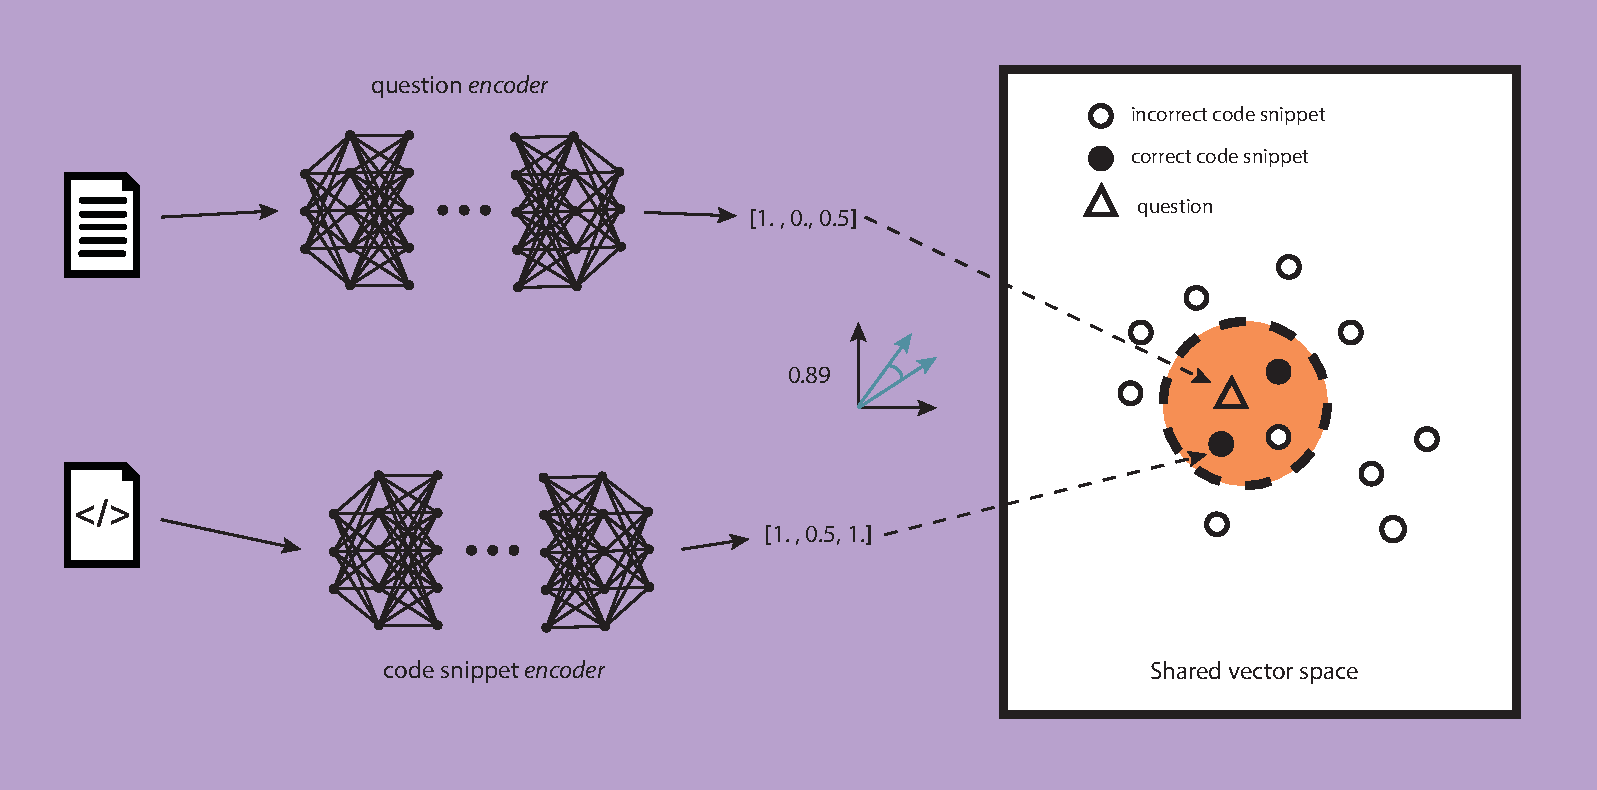
\includegraphics[width=\textwidth]{figuras/joint_embedding-article.pdf}
  \caption{Illustration of \emph{joint embedding} technique for code retrieval. Two neural networks map a question and a code snippet into a common vector space. The distance between the vectors reflects the relevance of a code snippet to a question.}
  \Description{None}
  \label{fig:joint-embedding}
\end{teaserfigure}

%%
%% This command processes the author and affiliation and title
%% information and builds the first part of the formatted document.
\maketitle

\section{Introduction}

The advent of open source code and open-domain question answering sites related to programming contributed to improve the way developers code today. Nowadays, code search is a daily routine task at software development process. Developers spend 15\% of their time searching for how a code works, a bug fix and API's usage \cite{what-developers-search-for-on-the-web:xia:2017}. According to \cite{sadowski-how-developers-search-for-code-case-study:2015}, developers at Google search for code 12 times a day, clicking on 2 to 3 results by average per search session. Most of them are looking for code examples. Thus, improve the way developers find a code it's an important productivity tool.  

Most of developers use general purpose search engine (GPSE) to look for code (e.g. Google). GPSE uses page rank and other indexes tactics that are not optimized for searching code. Then, GPSE are not capable of finding a code semantically, unless a code has a accompanying description. According to \cite{masudur-developers-use-google-code-retrieval:2018}, developers spend more time, visit more pages and change a query more often when they are doing a code-related search.

GitHub, a popular souce code hosting platform, have tried to build a semantic code search. They extracted millions of lines of code from its repositories and matched each code to a dosctring. The final results weren't satisfactory, the tool could find a relevant code only if we provide a query that matches the docstring description \citep{husain-github-semantic-search-code-2019}. According to \cite{cambronero-deep-code-search-2019}, a user's intent were better matched to questions collected from open-domain question-answering sites related to programming, e.g., StackOverflow. Those sites allow users to ask a question and approve the best answer for it. Other users can vote for the most helpful answer and mark the wrong or not helpful ones. Those collective actions help to curate and organize information, creating an important source of data.

Code search firts works were based on deductive-logic rules and manuallly extracted features \cite{Allamanis:2018:SML}. The recent success of artificial neural networks, due to Big Data and computational resources available, shifted recent works to a machine learning based approach. \cite{cambronero-deep-code-search-2019} also coined a name, neural code search, i.e., code search based on neural networks.

Recent works applied neural networks to summarize and retrieve code snippets. Code summarization and retrieval are two different tasks, each one has its metrics and traits. In our case, we are proposing a novel approach just for code retrieval. Our approach is based on Convolutional Neural Networks (CNN), while \cite{cambronero-deep-code-search-2019} proposed a neural networks with attention mechanism and \cite{Gu-deep-code-search:2018} presented a recurrent neural networks. \cite{cambronero-deep-code-search-2019} and \cite{Gu-deep-code-search:2018} paired code snippets and docstring, we matched code to questions collected from StackOverflow.

\subsection{Contributions of this work}

We can summarize the shortcomings of the existing work: most of neural networks approaches summarize and retrieve a code, although each one has its idiosyncrasy. As far as we know, we are the first to apply convolutional neural networks to search for code, due to good results in answer selection tasks \citep{feng-2015, wen-joint-modeling-question-answer-2019}. Recent works paired code and docstring, even though docstring doesn't match user's intent. Our research are trying to address each of these in turn by proposing and analyzing the CoNCRA, \emph{a Convolutional Neural Networks Code Retrieval Approach}.

\begin{itemize}
    \item We are proposing the CoNCRA, which is motivated
by the good results of convolutional neural networks at Natutal Language Processing (NLP) tasks. 
    \item We paired code and questions collected from StackOverflow. We used a new public available dataset created by \cite{yao-2018}.

    \item We evaluated the efficacy of our approach comparing to other methods: a baseline one and the actual state-of-the-art \cite{cambronero-deep-code-search-2019}.
    
\end{itemize}







\section{Methodology}
\label{sec:methodology}

According to \cite{cambronero-deep-code-search-2019}, the main goal of code retrieval is:

\emph{Retrieve code snippets from a code corpus that most closely match a developer's intent, which is expressed in natural language.}

The firsts works for code search used tools based on deductive-logic rules and manually extracted features. Deductive-logic approach, e.g. boolean model, finds a code that matches exactly the keywords expressed in the query. According to \cite{yan-benchmark-code-search-information-retrieval-deep-learning:2020}, those approaches are good at finding API's call and error's message, but it struggles to find reusable code and examples that don't have a exactly match between the code and query. Thus, there is a need to look for a semantic code search.

Neural networks showed good results at translation, question-answering and classifications tasks in NLP, it could infer words semantic and phrases context. Then, most of recent works adopted neural networks approach. \cite{cambronero-deep-code-search-2019} coined a term, \emph{neural code search}, searching for code using neural networks.

Recent works share a common strategy for code search, their approaches try to discriminate relevant code snippets from non-relevant one's based on an user's intent. In pursuance of that, code retrieval are reduced to a ranking problem where neural networks should be able to place code snippets that closely match developer's intent in the firsts ranks. The most common strategy to do that is \emph{joint embedding}. Joint embedding maps heterogeneous data into a common vector space, where the distance between embedded input reflects the similarity between the underlying items \cite{li-joint-embedding-images-2015} (see Figure~\ref{fig:joint-embedding}).

In order to apply joint embedding, 3 (three) items had to be considered:

\begin{itemize}
    \item Word embedding
    \item Sentence embedding
    \item Joint embedding
\end{itemize}

Embedding refers to a continuous vector in a lower dimensional vector space. A function that maps an input to a continuous vector is called \emph{encoder}. So, given an input set $X$, an encoder function $F$ can be defined as \cite{cambronero-deep-code-search-2019}:

\begin{equation}
    F: X \to E
\end{equation}

In our case, $X$ can be a set of questions or code snippets and $E$ is a set of continuous vectors or embeddings, such that $E \subset R^{d}$, where $d$ is the dimension. Our main goal is to learn two encoders $F$ and $G$ that maps a question and a code snippet, respectively, into a common vector space, so that the distance between the vectors reflect the relevance of a code snippet to a question (see Figure~\ref{fig:joint-embedding}). In our work, we are suggesting a convolutional neural networks approach to learn the sentence embedding, i.e., a convolutional neural networks will encode the question and code snippet into a continuous vector in a shared vector space. We also had to define how words are embedded and what objective function we are going to use, as the objective function tells how neural networks should approximate questions and code snippets.

\subsection{Word embedding}

The words and terms of a question and code snippet must be encoded into a numeric vector. The way those vectors are created it's very important, as a good vector will help neural networks to learn easily a task. The most common encoder for words is \emph{word2vec}, which embeds a word into a continuous vector based on distributional hypothesis. The distributional hypothesis says two words are similar if they appear together frequently in differents contexts \citep{Goodfellow-et-al-2016}. Context can be a sentence, paragraph or a document in NLP tasks. In our case, it's questions and code snippets.

Word2vec has two strategies: continuous-bag-of-words (CBoW) and skip-gram. The main difference between them is that CBoW predicts a target word given a context words and skip-gram predicts the context words given a single word. According to \cite{mikolov2013distributed}, CBoW showed good results at syntactically tasks, e.g., finding a superlative of a word or identify an adverb, while skip-gram presented a good performance at semantic tasks, e.g., finding the capital of a state or grouping feminine and masculine words. 

In our work, we opted for skip-gram as a semantic trait is preferable to a syntact one in our task. Semantic trait can help the neural networks to discriminate conditional clauses (e.g. \emph{if}, \emph{elsif}) and loop iteration (e.g. \emph{for}, \emph{while}), for an example. Figure~\ref{fig:tsne-code-snippet-python} shows an application of word2vec in a Python related corpus. If we look carefully, we can see the similarities between \emph{file}, \emph{write} and \emph{open}, as \emph{set}, \emph{list} and \emph{dict} based on the distance between them.

\begin{figure}[H]
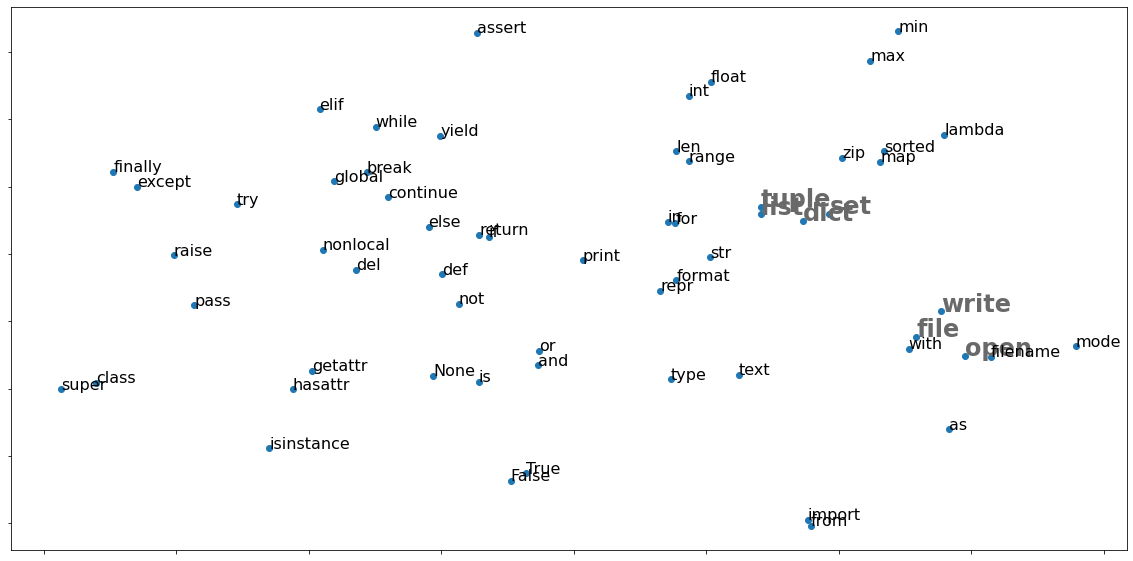
\includegraphics[width=0.45\textwidth]{figuras/code_tsne.png}
\caption{2D picture of continuous vectors of the 66 most frequent words from a Python corpus $V$. The illustration was generated by t-SNE, which allows 2D visualization from high-dimensional data. We applied word2vec with skip-gram and a parameter window $5$.}

\label{fig:tsne-code-snippet-python}
\end{figure}

\subsection{Sentence embedding}

We can combine the word embeddings to obtain a sentence embedding. Our proposal is to combine word embeddings by using a convolutional neural networks. Convolutional neural networks showed good results at answer selection task in NLP, where given a question and a set of answers, the model should rank the best answers in the firsts positions. Although, convolutional networks prioritizes local interactions (e.g. words nearby) and can't capture long range dependencies (e.g. distant words in a sentence), we think it does not represent a big problem to code retrieval, as most of questions and code snippets are short in length.

Given an sentence $\bm{x} = \{ \bm{x}(0), \bm{x}(1), . . ., \bm{x}(n - 1) \}$, such that $\bm{x}(i) \in \mathbb{R}^{d}$ is a continuous vector that represents the $i^{th}$ word of the sentence. The convolutional neural networks combines the elements of vector $\bm{x}$ by applying 2 basic operations:

\begin{itemize}
    \item Convolution operation
    \item \textit{Maxpool}
\end{itemize}

A convolution operation uses a filter $\bm{F}  = [\bm{F}(0),· · ·, \bm{F}(m - 1)]$, such that $\bm{F} \in \mathbb{R}^{m X d}$. The operation applies the filter in $m$ words (window size) in order to produce a new vector. Suppose $\bm{x}(i, i + j)$ refer to a concatenation of the vectors $\bm{x}(i), \bm{x}(i + 1), . . ., \bm{x}(i + j)$. If we apply $\bm{F}$ to $\bm{x}(i, i + m - 1)$, then we can calculate a new vector $\bm{c}(i)$ by:

\begin{equation}\label{eq:calc_convolution_ci}
    \bm{c}(i) = tanh \left[\left(\sum_{j=0}^{m - 1} \bm{x}(i + j)^{T}\bm{F}(j)\right) + b\right]
\end{equation}

In the equation~\ref{eq:calc_convolution_ci}, $\bm{F}$ and $b$ are learnable weights and bias, respectively. The convolution operation slides the filter $\bm{F}$ across the height of input $\bm{x}$ and computes the dot product between the entries of the filter and the input \cite{karpathy-course-cnn-2016}. The operation returns a feature map $\bm{c}$.

\begin{equation}
    \bm{c} = \{ \bm{c}(0), \bm{c}(1), . . ., \bm{c}(n - m) \} 
\end{equation}

The feature map (or activation map) contains the latent and most important features of a sentence. A convolutional neural networks may contain thousands of filters, each one extracting specific \emph{m-gram} features. A filter of $m$ size 2 extracts bigram features, a size of 3 extracts trigram features, and so on. The quantity of feature maps is $|F|$, i.e., the number of filters. After the convolution operation, a pooling layer operates independently on every feature map resizing it spatially, using a max operation \cite{karpathy-course-cnn-2016}.  The max operation is applied along the $axis=0$ to produce the final vector $\bm{o}$:

\begin{equation}
    \bm{o} = max\left(\left[\bm{c}_{1}, \bm{c}_{2}, . . ., \bm{c}_{|F|}\right], axis = 0\right)
\end{equation}

The max pooling helps the convolutional neural networks to be translation invariant. Regardless of the word's position shift, the max pooling selects the most relevant features and insert into the final vector \citep{tom-young:trends-deep-learning-nlp}. Figure~\ref{fig:cnn-steps-word-embedding} shows the results of each operation. We use the vector $\bm{o}$ as our sentence embedding, then $\bm{o}$ represents a question or a code snippet, in our case. 

\begin{figure}[H]
    \centering
    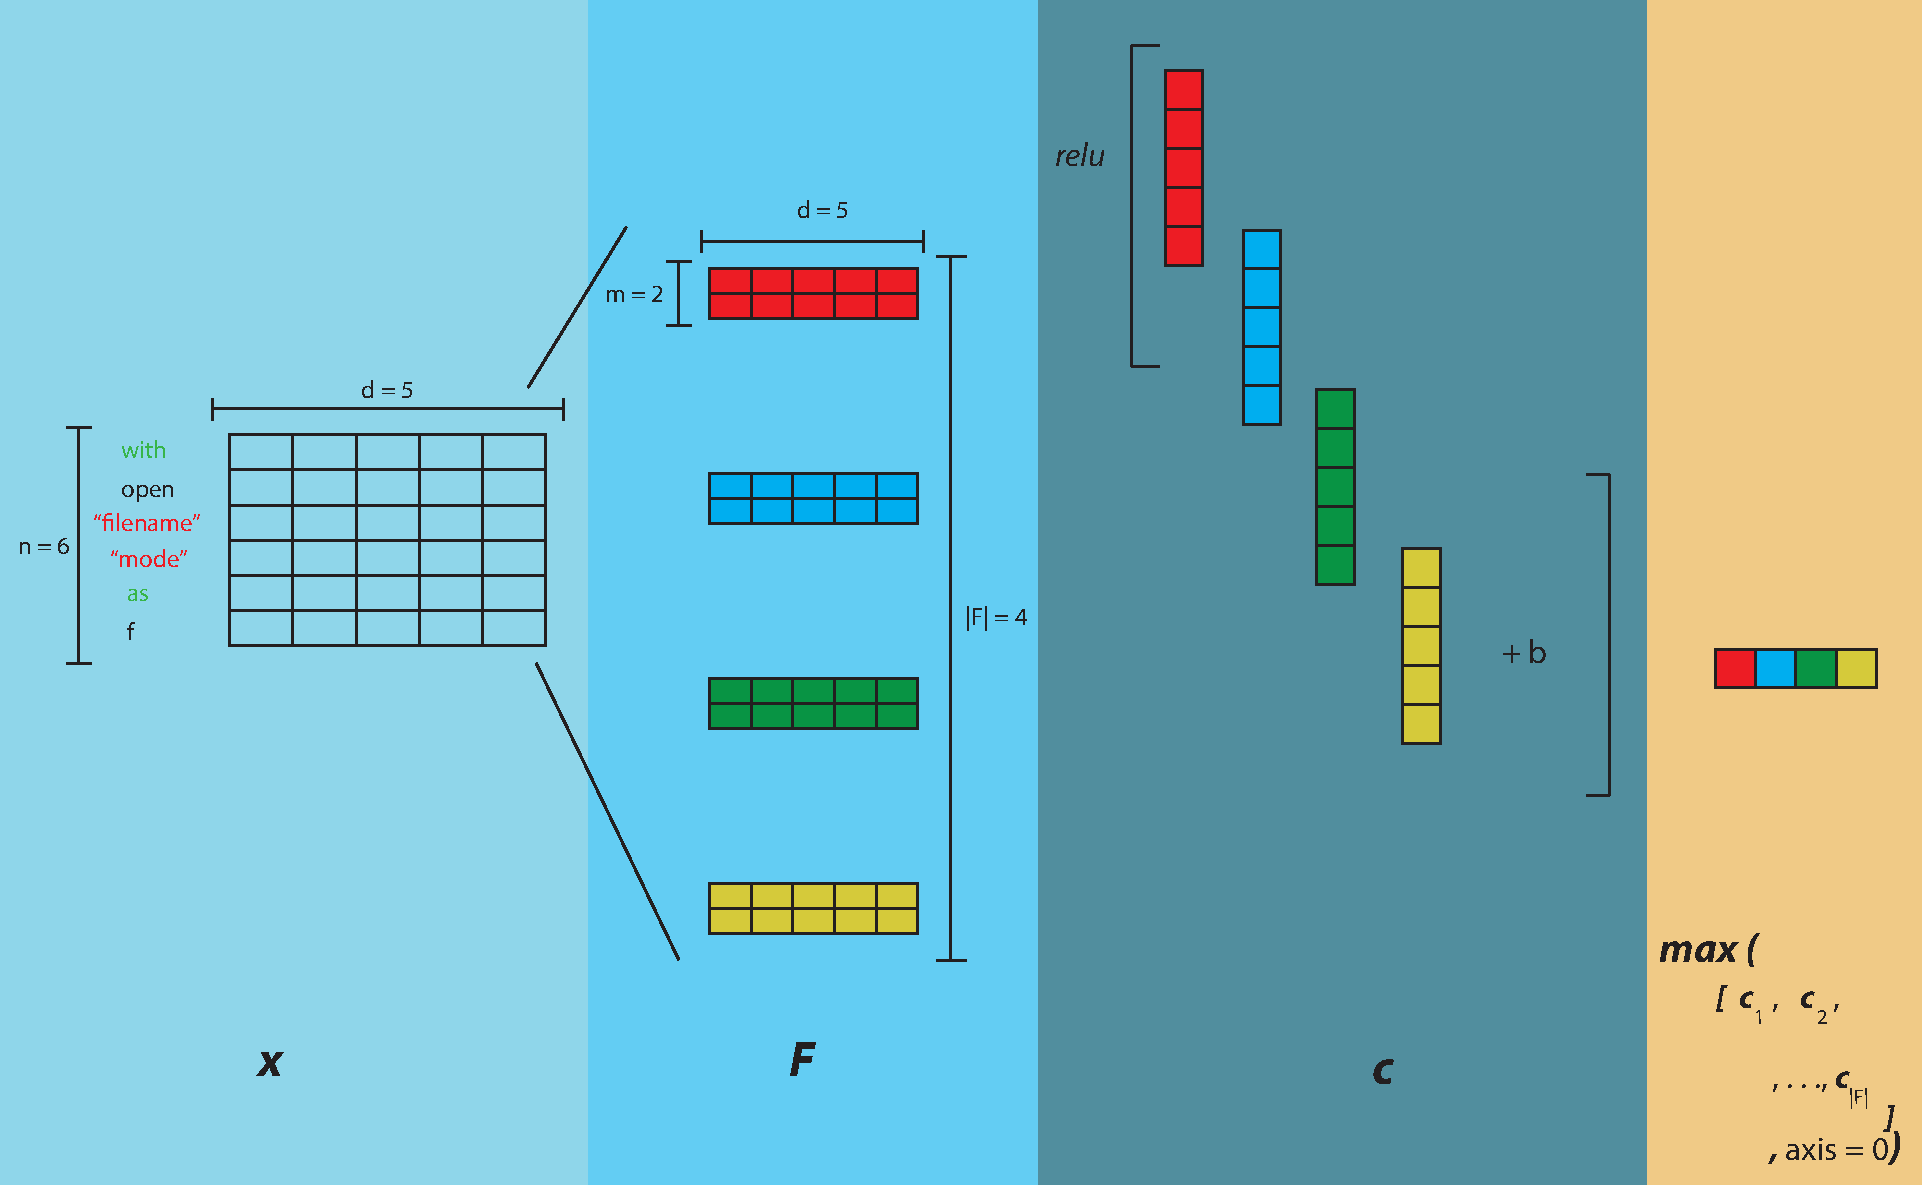
\includegraphics[width=0.45\textwidth]{figuras/cnn-steps-word-embedding-article.pdf}
    \caption{Schematic drawing of our Convolutional Neural Networks (CNN) operation results. Our example shows 4 filters $\bm{F} \in \mathbb{R}^{m X d X f}$ with window size $m = 2$. We slide each filter across the height of the input $\bm{x} \in \mathbb{R}^{n X d}$, where $n = 6$ and $d = 5$, and computes the dot product between the entries of the filter and the input \cite{karpathy-course-cnn-2016}. It returns a feature map $\bm{c}$. In the end, a max pooling layer resizes every feature map spatially, obtaining the final vector $\bm{o}$. We use the vector $\bm{o}$ as our question and code snippet embedding. Adapted from \cite{zhang-guide-convolutional-cnn-embedding-ilustration:2015}.}
    \label{fig:cnn-steps-word-embedding}
\end{figure}

\subsection{Joint embedding}
\label{sec:joint-embedding}

In our work, we reduced code retrieval to a ranking problem, where a model should rank a relevant code in the firsts positions based on a developer's intent. In order to do that, we choose an objective function that prioritizes the relative preference of the code snippets, instead of a correct classification. The objective function, in our case, helps the neural networks to discriminate the correct answers from incorrect ones during the training phase.


Given a question and code snippet set, $\mathbb{Q}$ and $\mathbb{C}$, our training input is composed by a triple $<\bm{q}, \bm{c^{+}}, \bm{c^{-}}>$, where $\bm{c^{+}} \in \mathbb{C}$ indicates a correct code snippet for a question $\bm{q} \in \mathbb{Q}$ and $\bm{c^{-}} \in \mathbb{C}$ its an incorret one sampled from the training data. We used the hinge loss as our objective function. Formally, for a triple $<\bm{q}, \bm{c^{+}}, \bm{c^{-}}>$, the definition of hinge loss is:

\begin{equation}
J = max(0, m - h_{\theta}(\bm{q}, \bm{c^{+}}) + h_{\theta}(\bm{q}, \bm{c^{-}}))
\end{equation}

$m$ its a margin and $h_{\theta}$ its a similarity function (e.g., \textit{cosine}). During the training phase, the goal is to minimize the cost function $J$. In order to obtain that, the model aims to satisfy the following condition: $h_{\theta}(\bm{q}, \bm{c^{+}}) - h_{\theta}(\bm{q}, \bm{c^{-}}) \geq m$. Then, the hinge loss function induces our model to score $c^{+}$ higher than $c^{-}$ for a given margin $m$. 

For the similarity function $h_{\theta}$, we used \emph{cosine}, such that $h_{\theta}(\bm{q}, \bm{c}) = \{h_{\theta}(\bm{q}, \bm{c}) \in \mathbb{R} | 0 \leq h_{\theta}(\bm{q}, \bm{c}) \leq 1$\} computes the similarity between the vector $\bm{q} \in \mathbb{Q}$ and $\bm{c} \in \mathbb{C}$. $0$ indicates orthogonality e $1$ indicates greater similarity \cite{keras-cosine-similarity-2019}.  Given that our objective function aims to satisfy the following condition: $h_{\theta}(\bm{q}, \bm{c^{+}}) \geq h_{\theta}(\bm{q}, \bm{c^{-}}) + m$. Thus, we are inducing our model to group $\bm{c^{+}}$ and $\bm{q}$ nearby, while the vectors $\bm{c^{-}}$ would be far away (see Figure~\ref{fig:joint-embedding}). 

\section{Experiments}

We evaluated our proposed approach (CoNCRA) on StaQC dataset, a systematically mined question code dataset from StackOverflow \cite{yao-2018}. The main difference of StaQC to other datasets is it is composed by ''how-to-do-it'' questions, as most of the answers to those type of questions are straight. StaQC contains SQL and Python question and code pairs, but, in our preliminary experiment, we used the Python ones only. Table~\ref{table:summary-training-data-yao-staqc} shows a summary of StaQC dataset.

\begin{table}[h]
\centering
\begin{tabular}{ p{5cm} c c }
\hline
  & \multicolumn{2}{c}{\textbf{Question}}\\
\hline
\textbf{Code snippet} & \textbf{Python} & \textbf{SQL}  \\
\hline

$N_{1}$: Single code snippet in the answer description & $85.294$ & $75.637$ \\

$N_{2}$: Automatically annotated code snippets & $60.083$ & $41.826$ \\

$N_{3}$: Manually annotated code snippets & $2.169$ & $2.056$  \\

 \hline
 \textbf{Total} & $\bm{147.546}$ & $\bm{119.519}$\\
 \hline 
 
\end{tabular}
\caption{Summary of StaQC dataset \cite{yao-2018}. Questions from $N2$ sample ("Automatically annotated code snippets") may contain more than one code snippet per answer description. Some code snippets may not be a solution for the question. So, the authors proposed a framework to annotate the code snippets automatically and it could achieve a F1 score of $0,916$ and an accuracy of $0,911$.}
\label{table:summary-training-data-yao-staqc}
\end{table}

\begin{table}[h]
\centering
\begin{tabular}{ l r  }
 \hline
 \textbf{Sample} & \textbf{Quantity of pairs $<q_{i}, c_{i}^{+}>$}\\
 \hline
 $N_{2} = \text{Training}$ & $60.083$\\
 
 $N_{3} \supset \text{DEV}$ & $1.085$ \\
 
 $N_{3} \supset \text{EVAL}$ & $1.084$\\
 \hline
 \textbf{Total} & $\bm{62.252}$\\
 \hline
\end{tabular}
\caption{Summary of our training and evaluation samples. The samples are composed by a pair $<q_{i}, c_{i}^{+}>$, where $q_{i}$ its a question and $c_{i}^{+}$ its a code snippet annotated as solution. We spplited the manually annotated dataset in two parts: DEV and EVAL, according to \cite{iyer-etal-2016-summarizing} procedure. }
\label{table:training-sample-division}
\end{table}

We trained our model on sample $N2$ (see Table~\ref{table:summary-training-data-yao-staqc} and Table~\ref{table:training-sample-division}), because 27\% of the questions contains more than one answer annotated, leading to more variance in our training dataset. The training and evaluation follows the \cite{iyer-etal-2016-summarizing} procedure, where the model is evaluated on an manually annotated dataset each epoch according to a Mean Reciprocal rank (MRR). The MRR tells if a model ranked the annotated answer in higher positions, i.e., higher values for MRR indicates the accepted answers were ranked in the firts positions.

For the training phase, we spplited 70\% of $N2$ sample for training and 30\% for validation. We run the models for 500 epochs and stops early if the training loss ($J$) is less than $0.0001$ or the validation loss doesn't improve after 25 consecutive epochs. For the final evaluation, we choose the best model of the training phase according to MRR and run it for 20 iterations in the $N3$ sample (see Table~\ref{table:training-sample-division}). The final result is the average of the MRR for each pair $<q_{i}, c_{i}^{+}>$ of $N3$ and other 49 distractors $c_{j}$, which were selected randomly from the training sample, such that $c_{i}^{+} \neq c_{j}$.

 We provided the source code for our preliminary experiments in the following repository: \url{https://github.com/AUTHOR/PROJECT_NAME}. The repository contains our proposed model, the baseline ones, training and evaluation source code. We also provided the original and pre-processed dataset. The source code is written in Python, version 3.6.9, and we used the libraries Keras (version 2.2.4-tf) and Tensorflow (1.15.2). The preliminary experiments were all conducted in the Colab, a Google platform that allows to run arbitrary Python code from the browser and it's specially suited for machine learning and data analysis research \cite{colab-2019}.

\subsection{Results}

For the final evaluation, we compared the following models:

\begin{itemize}
    \item \emph{CoNCRA}: our proposed approach described in the Section~\ref{sec:methodology}. We tried two variations of our approach, the Convolutional Neural Networks (CNN) and Shared CNN. The main difference between them is that Shared CNN shares the weights through the process of learning the question and code snippet embeddings, while CNN learns different weights for each one.
    \item \emph{Embedding}: it's our baseline model. It's a simple architecture that applies a max pooling layer to the word embeddings. 
    \item \emph{Unif}: it's a architecture proposed by \cite{cambronero-deep-code-search-2019}. They used two distinct layers for the question and code snippet embedding. They applied an average pooling layer to word embedding in order to learn the question embeddings. For the code snippet, they used an attention mechanism, which applies a weighted average to each word embedding, ''giving an attention'' to the most relevant word of the code.
\end{itemize}

All the models used the joint embedding technique described in the Section~\ref{sec:joint-embedding}. Table~\ref{table:resultados} shows the final results we got after 20 runs on the $N3$ sample. Shared CNN with 4000 filters got the best results (lines D3 e F3). Our proposed architecture achieved a MRR score 5\% higher on average than the best result obtained by Unif (linha B1), actual state-of-the-art. Our MRR result is 11\% higher than the baseline model (linha A1). 

\begin{table*}[t]
\centering
\begin{tabular}{ p{1cm} p{6cm} >{\raggedleft\arraybackslash}p{4cm} >{\raggedleft\arraybackslash}p{4cm} }
 \hline
    & & \multicolumn{2}{c}{\textbf{Results}}\\
 \hline
 & \textbf{Models} & \textbf{MRR} & \textbf{TOP-1}\\
 \hline
 A1 & Embedding (m = $0.1$) & $0.637$& $0.493 \pm 0.009$\\
 
 \hline
 
 B1 & Unif (m = $0.2$) & $0.675 \pm 0.006$ & $0.539 \pm 0.009$\\
 
 \hline
 
 C1 & CNN / F = 1000 & $0.669 \pm 0.006$ & $0.527 \pm 0.012$\\
 
 C2 & CNN / F = 2000 & $0.673 \pm 0.007$ & $0.531 \pm 0.012$\\
 
 C3 & CNN / F = 4000 & $0.687 \pm 0.006$ & $0.553 \pm 0.011$\\
 
 \hline
 
 D1 & Shared CNN / F = 1000 & $0.678 \pm 0.007$ & $0.548 \pm 0.012$\\
 
 D2 & Shared CNN / F = 2000 & $0.694 \pm 0.008$ & $0.565 \pm 0.012$\\
 
 D3 & Shared CNN / F = 4000 & $0.700 \pm 0.004$ & $0.569 \pm 0.009$\\
 
 \hline
 
 E1 & CNN with BN / F = 1000 & $0.682 \pm 0.007$ & $0.543 \pm 0.012$\\
 
 E2 & CNN with BN / F = 2000 & $0.689 \pm 0.006$ & $0.553 \pm 0.011$\\
 
 E3 & CNN with BN / F = 4000 & $0.688 \pm 0.006$ & $0.553 \pm 0.011$\\
 
 \hline
 
 F1 & Shared CNN with BN / F = 1000 & $0.690 \pm 0.008$ & $0.553 \pm 0.015$\\
 
 F2 & Shared CNN with BN / F = 2000 & $0.700 \pm 0.007$ & $0.573 \pm 0.012$\\
 
 F3 & Shared CNN with BN / F = 4000 & $0.701 \pm 0.008$ & $0.577 \pm 0.015$\\
 
\hline
\end{tabular}
\caption{The experimental results of EVAL sample for Embedding, Unif and our two CNN variations: CNN and Shared CNN. \emph{m} refers to margin loss of the hinge loss function (lines A1 and B1). \emph{F} indicates the quantity of filters. BN its an acronym of Batch Normalization. Our CNN architecture used a margin loss $m = 0.05$ and a window size $2$.}
\label{table:resultados}
\end{table*}

According to Table~\ref{table:resultados}, an increase in the number of filters results in a better performance for CNN, as the model capacity and the number of extracted features grow (lines D3 e F3). 
We tried different margin loss (see Section~\ref{sec:joint-embedding}), CNN got the best results with  $0.05$, while Unif and Embedding got better results with $0.2$ and $0.1$, respectively. 


We verified that shared weights models (lines D e F) got better results than independently weights ones (lines C e E). One reason is that the optimizer of independently weights architecture has to learn the double of parameters, increasing the learning difficulty \cite{feng-2015}. We also tried a batch normalization technique to avoid overfitting and help our models to learn quickly and more stable, but only CNN and Shared CNN got better results. For Unif and Embedding, it didn't improve the performance at all. 

The Figure~\ref{fig:histogram-mrr} illustrates the MRR (Mean Reciprocal Rank), showing the first position of the annotated code snippet during the final evaluation.

\begin{figure}[H]
    \centering
    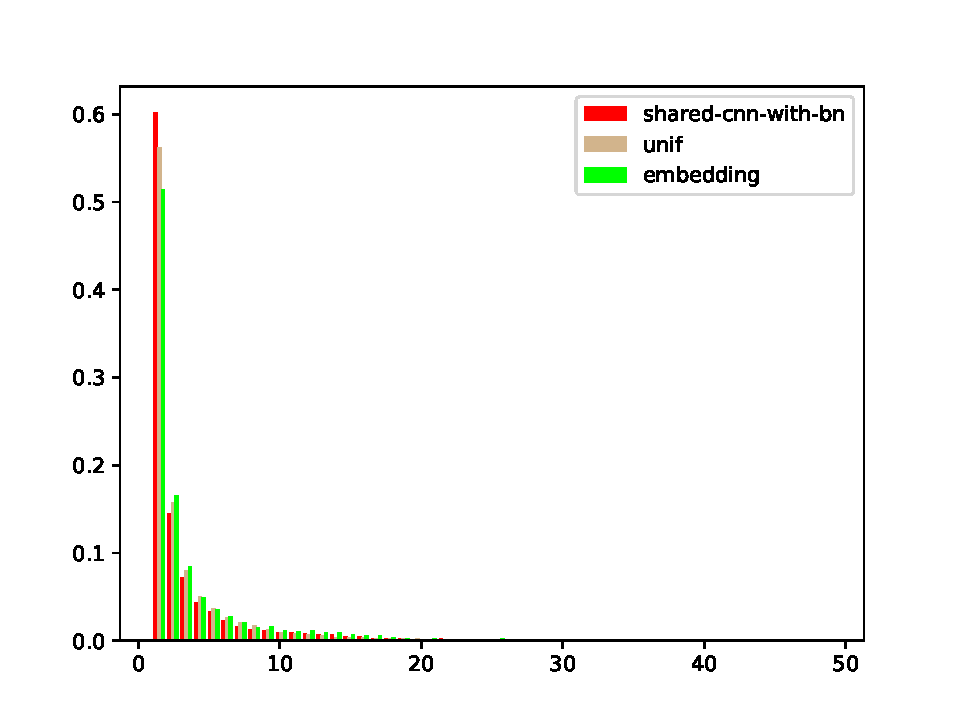
\includegraphics[width=0.45\textwidth]{figuras/histogram.pdf}
    \caption{Histogram of the firsts positions observed for the annotated code snippet during the final evaluation. The labels \emph{shared-cnn-with-bn}, \emph{unif} and \emph{embedding} refer to lines F3, A1 e B1, respectively, in the Table~\ref{table:resultados}.}
    \label{fig:histogram-mrr}
\end{figure}


Both CNN and Unif ranked the code snippets among the first 3 positions in 75\% of cases. We got a TOP-1 accuracy of 60\%, i.e., we ranked the relevant code snippet first place in 60\% of cases. Unif and Embedding got a TOP-1 accuracy of almost 50\%. One thing to note however is that MRR takes only the position of the annotated code snippet into consideration. Then, if the model shows up another code snippet, which answers the question correctly, our metric doesn't take it into account. In the end, the model is penalized. 

\subsection{Threats to validity}

We trained the models on StaQC dataset, a systematically mined question code dataset. The authors used a neural networks to annotate the code snippet and trained it on a manually dataset. In our case, we trained the models on the automatically annotated corpus and evaluated on the manually ones. To mitigate the bias, we adopted the \cite{iyer-etal-2016-summarizing} procedure for training and evaluation.

\section{Conclusion}

According to results, our proposed approach is a prominent techique. Our model achieved a MRR score 5\% higher on average than Unif, actual state-of-the-art. We could rank the most relevant code snippet among the first 3 (three) positions in 78\% of cases. Our techique achieved a TOP-1 accuracy of 60\%, while the others techniques got 50\%. 

Although the results seems good, it's a preliminary experiment, a further investigation is needed to see if our model is invariant to others datasets. We also would like to try a transfer learning, e.g., check if a model trained on a StackOverflow dataset (curated corpus) is able to find relevant code snippets in a Github corpus (non-curated one). Our approach is based on a NLP technique proposed by \cite{feng-2015}, we think future works may use transformers and autoencoders, as those techniques showed good results in many NLP tasks. 

%%
%% The next two lines define the bibliography style to be used, and
%% the bibliography file.
\bibliographystyle{ACM-Reference-Format}
\bibliography{sample-base}

%%
%% If your work has an appendix, this is the place to put it.


\end{document}
\endinput
%%
%% End of file `sample-sigconf.tex'.
